\chapter{Flash Attention}

``\textit{Many approximate attention methods have aimed to reduce the compute and memory requirements of attention. These methods range from sparse-approximation to low-rank approximation, and their combinations. Although these methods reduce the compute requirements to linear or near-linear in sequence length, many of them do not display wall-clock speedup against standard attention and have not gained wide adoption. One main reason is that they focus on FLOP reduction (which may not correlate with wall-clock speed) and tend to ignore overheads from memory access (IO)}'' \cite{dao2022flashattention}.

\begin{itemize}
	\item    Fast — excerpt from the paper: "We train BERT-large (seq. length 512) 15\% faster than the training speed record in MLPerf 1.1, GPT2 (seq. length 1K) 3x faster than baseline implementations from HuggingFace and Megatron-LM, and long-range arena (seq. length 1K-4K) 2.4x faster than baselines."
	\item Memory-efficient — compared to vanilla attention, which is quadratic in sequence length, $O(N^2)$, this method is sub-quadratic/linear in $O(N)$. We'll see later why & how.
	\item Exact — meaning it's not an approximation of the attention mechanism (like \eg sparse, or low-rank matrix approximation methods) — its outputs are the same as in the "vanilla" attention mechanism.
	\item IO aware — compared to vanilla attention, flash attention is sentient.
\end{itemize}

Over the years GPUs have been adding compute capacity (FLOPS) at a faster pace than increasing the memory throughput (TB/s).

It doesn't matter if you can compute at exaFLOPS speeds if there is no data to be processed. These 2 need to be closely aligned, and since the hardware lost that balance we have to make our software compensate for it.

It turns out attention is (on current AI accelerators) memory-bound.
\begin{itemize}
	\item Softmax
	\item Dropout
	\item Masking
	\item Matmul
\end{itemize}




Modern GPUs have a strict memory hierarchy:
\begin{itemize}
	\item SRAM – fast, on-chip, small
	\item HBM – slower than SRAM, large size. That's what we usually address as GPU memory.
\end{itemize}
Every operation that "does math" must move data from HBM up to SRAM and then write results back. Those transfers are not free. For attention, the cost of reading and writing dominates; the kernels often become bandwidth/IO-bound rather than compute-bound.

The problem with the vanilla attention is that attention forms the full score matrix:
\begin{align*}
	S = \frac{QK^\top}{\sqrt{d_k}}
	% \operatorname{softmax}\left(\frac{QK^\top}{\sqrt{d_k}}\right)
\end{align*}
There are several issues:
\begin{itemize}
	\item Materialization of $S$: $S$ is a $N\times N$ matrix. For long sequences, just storing and moving $S$ overwhelms SRAM capacity and HBM bandwidth.
	\item SRAM limits: To compute the softmax for one query token $i$, you'd like all scores on chip.
\end{itemize}
In short: the IO pattern is wasteful.

FlashAttention makes attention IO-aware by restructuring computation to minimize reads/writes between HBM and SRAM while staying exact:
\begin{itemize}
	\item Tile the sequence: Load small blocks (tiles) of $Q, K$, and $V$ that fit in SRAM. Compute partial $QK^⊤$ for that tile only.
	\item Online/streaming softmax: For each query row $i$, keep tiny running statistics in SRAM
	\item Write once: When a row is complete (all tiles processed), write the final output to HBM. You avoid the ($O(N^2)$) intermediate traffic.
\end{itemize}

However, this matrix is necessary for transformer training as it is a part of backpropagation and gradient calculation. The authors propose that it's better to recalculate this matrix during the backward pass (again without explicit materialization). Not only does this saves lots of memory, but it also provides huge speedups as we don't need to transfer this enormous matrix between different GPU memory types.

Overall, such an approach did not only speed up calculations by taking GPU I/O specifics into account, but also allowed processing huge sequence lengths as memory complexity drops to $O(n)$.

In sum,
\begin{itemize}
	\item Load a small block of $Q$ and $K$ into SRAM.
	\item Compute just that block of scores ($Q\cdot K^T$).
	\item Do a streaming softmax: keep a running max and sum so softmax stays numerically stable without needing all tokens at once.
	\item Immediately apply that softmax block to the matching $V$ block and accumulate partial outputs.
	\item Move to the next tile. When all tiles are processed, you already have the final output—no big attention matrix ever stored.
\end{itemize}
This is called an IO-aware algorithm: it minimizes slow memory traffic and maximizes use of the GPU's fast memory.

What attention normally does (and why it's slow)

Given per-head matrices:
\begin{itemize}
	\item$Q \in \mathbb{R}^{N\times d}, K \in \mathbb{R}^{N\times d}, V \in \mathbb{R}^{N\times d_v}$ 
	\item Scores: $S = \frac{QK^\top}{\sqrt{d}}  (\text{size } N\times N)$
	\item Output: $O = \mathrm{softmax}(S)V$
\end{itemize}
Naive kernels materialize $S$ (size ($N^2$)), apply softmax row-wise, then multiply by $V$.
Problem: writing/reading ($N^2$) scores to HBM (GPU DRAM) is \textit{memory-bound} and explodes memory as $N$ grows (\eg $4k$ tokens $\to$ $16M (4k^2)$ scores per head).

The core idea of FlashAttention is to compute over tiles. If we compute matrix multiplications over small blocks or tiles, we can significantly reduce the amount of memory access.

However, to compute the attention scores, we still have to compute the softmax. To compute the softmax over tiles, we can adopt online softmax and never form $S$ in HBM. In other words, do attention in tiles that fit in on-chip SRAM to minimize HBC traffic, and keep only tiny per-row summaries in HBM. For each tile:

\begin{enumerate}
	\item Load a block of $Q$ and a block of $K$, $V$ into SRAM.
	\item Compute partial scores $S_{\text{blk}} = Q_{\text{blk}}K_{\text{blk}}^\top/\sqrt{d}$.
	\item Apply a streaming softmax update so you don't need the whole row at once.
	\item Immediately multiply by $V_{\text{blk}}$ and accumulate partial
		outputs for that row block.
	\item Move to the next block of $K/V$ and repeat.
\end{enumerate}

\begin{figure}[t]
	\centering
	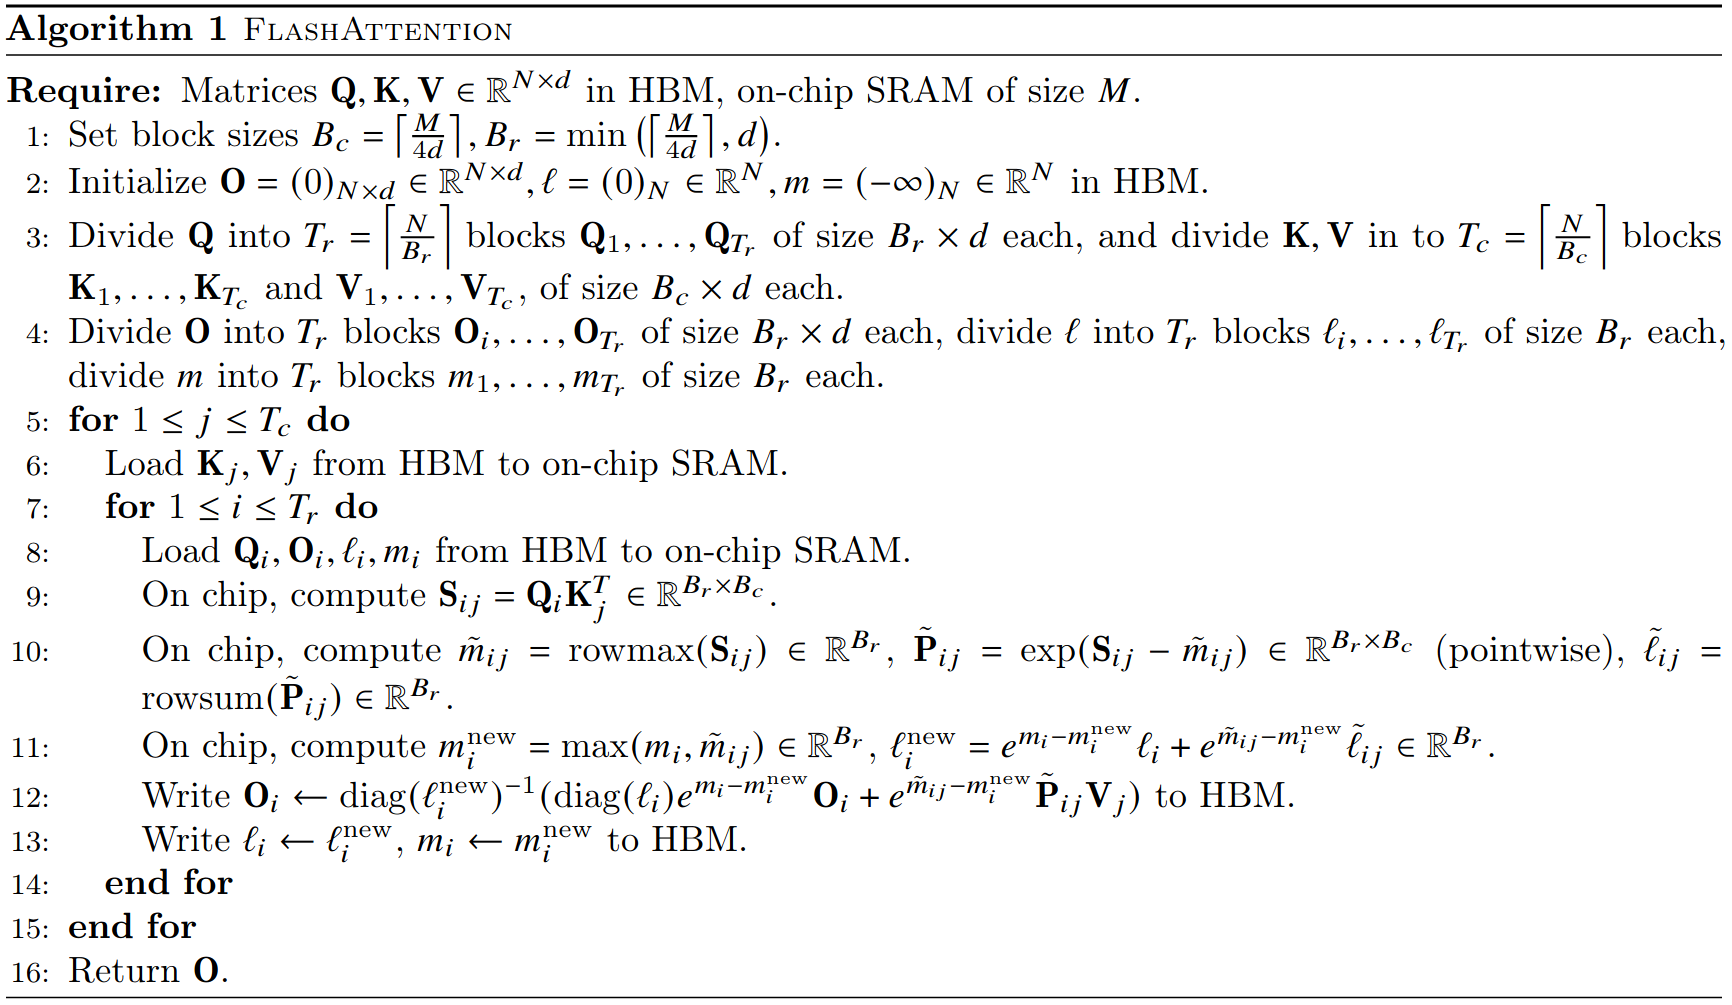
\includegraphics[scale=0.45]{./images/flash_attn.png}
\end{figure}
\begin{itemize}
	\item $\frac{M}{4d}$: Note that query, key, and value vectors are $d$-dimensional. We also need to combine them into the $d$-dimensional output vector. To load all four vectors, it has to be $4d$.
\end{itemize}


\section{The streaming (online) softmax trick}

Note that a naive implementation of softmax can suffer from overflow issue, since softmax uses exponentials, and exponentials blow up (or vanish) fast. The standard way to fix this issue is to shift by the max (\ie log-sum-exp trick).

Softmax is shift-invariant:
\begin{align*}
	\mathrm{softmax}(x)_i = \mathrm{softmax}(x - c)_i \quad \text{for any constant } c.
\end{align*}
Choose $c = m = \max_j x_j$. Define $\tilde{x}_i = x_i - m \le 0$. Then
\begin{align*}
	\mathrm{softmax}(x)_i
	= \frac{e^{x_i - m}}{\sum_j e^{x_j - m}}
	= \frac{e^{\tilde{x}_i}}{\sum_j e^{\tilde{x}_j}}.
\end{align*}

For one output row $i$ ($i$-th query token), the softmax over all keys $j=1\ldots N$ is:
\begin{align*}
	o_i = \sum_{j=1}^N \frac{e^{s_{ij}}}{\sum_{k=1}^N e^{s_{ik}}} v_j,
	\quad s_{ij} = \frac{q_i\cdot k_j}{\sqrt{d}} + \text{mask/bias}.
\end{align*}
To compute how much a particular $i$-th token from the input sequence pays attention to other tokens in the sequence,  you'd need to have all of those scores (\ie denominator) readily available (denoted here by $s_{ij}$) in SRAM. However, SRAM is limited in its capacity. Thus, we process keys in chunks (\ie tiles). Maintain per-row running stats. In other woreds, We process keys $j=1,\dots,N$ in chunks (tiles). For each row $i$ keep running statistics:
\begin{itemize}
	\item $m_i$: running max score seen so far (for numerical stability)
	\item $\ell_i$: running sum of exp-shifted scores, \ie $\ell_i = \sum e^{s_{ij}-m_i}$
	\item $z_i$: running weighted sum of values, $z_i = \sum e^{s_{ij}-m_i} v_j$
\end{itemize}
When you see a new block with per-row block max $m_i^{\text{blk}}=\max_j s_{ij}^{\text{blk}}$ and sums
\begin{itemize}
	\item $\ell_i^{\text{blk}} = \sum_j e^{s_{ij}^{\text{blk}}-m_i^{\text{blk}}},$
	\item $z_i^{\text{blk}} = \sum_j e^{s_{ij}^{\text{blk}}-m_i^{\text{blk}}} v_j,$
\end{itemize}
update with running stats:
\begin{align*}
	m_i^{\text{new}} &= \max(m_i, m_i^{\text{blk}}),\\
	\ell_i^{\text{new}} &= \ell_i e^{m_i - m_i^{\text{new}}}
	+
	\ell_i^{\text{blk}} e^{m_i^{\text{blk}} - m_i^{\text{new}}},\\
	z_i^{\text{new}} &= z_i e^{m_i - m_i^{\text{new}}}
	+
	z_i^{\text{blk}} e^{m_i^{\text{blk}} - m_i^{\text{new}}}.
\end{align*}
At the end of all blocks:
\begin{align*}
	o_i = \frac{z_i}{\ell_i}.
\end{align*}
classic log-sum-exp fusion with dynamic max shifting keeps numbers well-scaled without needing all $s_{ij}$ at once.


\begin{commentbox}{Example}
\begin{itemize}
	\item scores (two tiles): $s=[1,3|0,2]$
	\item 2-D values:
		\begin{itemize}
		  \item (v_1=[1,0])
		  \item (v_2=[0,2])
		  \item (v_3=[-1,1])
		  \item (v_4=[3,1])
		\end{itemize}
\end{itemize}
Define $a=e^{-2}\approx0.135335, b=e^{-1}\approx0.367879$.

\begin{itemize}
	\item \textbf{Tile 1}: $[1,3]$ with$[v_1,v_2]$ 
		\begin{itemize}
			\item block max: $m^{\text{blk}}=3$ 
			\item block sums (shift by $m^{\text{blk}}$):
				\begin{align*}
					\ell^{\text{blk}} &= e^{1-3}+e^{3-3} = a+1\\
					z^{\text{blk}} &= av_1 + 1\cdot v_2
					  = a[1,0]+[0,2] = [a,,2]
				\end{align*}
			\item merge into running stats (start from $m=-\infty,\ell=0,z=0$):
				\begin{align*}
					  m\leftarrow 3,\quad \ell\leftarrow a+1,\quad z\leftarrow [a,2].
				\end{align*}
		\end{itemize}
	\item \textbf{Tile 2}: $[0,2]$ with$[v_3,v_4]$ 
		\begin{itemize}
			\item block max: $m^{\text{blk}}=2$ 
			\item block sums:
				\begin{align*}
				  \ell^{\text{blk}}=a+1,\quad
				  z^{\text{blk}}=av_3+1\cdot v_4
				  = a[-1,1]+[3,1] = [3-a,1+a].
				\end{align*}
			\item merge (global max stays $m^{\text{new}}=\max(3,2)=3$):
				\begin{align*}
					\ell &\leftarrow \ell\cdot e^{3-3} + \ell^{\text{blk}}\cdot
					e^{2-3} = (a+1) + (a+1),b \approx \boxed{1.55300179}\\
				  z &\leftarrow z\cdot e^{3-3} + z^{\text{blk}}\cdot e^{2-3}
				  = [a,2] + b[3-a,1+a] \approx \boxed{[1.18918654,2.41766651]}.
				\end{align*}
		\end{itemize}
	\item \textbf{Finalize} (elementwise divide by scalar $\ell$)
		\begin{align*}
			o=\frac{z}{\ell}
			\approx \Big[\frac{1.18918654}{1.55300179},\frac{2.41766651}{1.55300179}\Big]
			= \boxed{[0.76573417,1.55676994]}.
		\end{align*}
	\item \textbf{Sanity check} (plain softmax on all 4 keys)
		Weights from $s=[1,3,0,2]$ are $\approx[0.08714,,0.64391,,0.03206,,0.23688]$.
		\begin{align*}
			\sum_j w_j v_j
			&= 0.08714[1,0]+0.64391[0,2]+0.03206[-1,1]+0.23688[3,1]\\
			&= [0.76573417,1.55676994],
		\end{align*}
		which matches the streaming result exactly. 
\end{itemize}
\end{commentbox}

% \begin{lstlisting}[language=Python]
% # Q: [nq, d], K: [nk, d], V: [nk, dv]
% # Tile sizes chosen so a Q tile and a K/V tile fit in SRAM.
% m = -inf * ones(nq)        # running max per row
% l = zeros(nq)              # running sum-exp per row
% z = zeros(nq, dv)          # running weighted sum per row

% for each KV_tile in partition_along_keys(K, V):
%     Kb, Vb = KV_tile  # [tk, d], [tk, dv]
%     for each Q_tile in partition_along_queries(Q):
%         Qb = Q_tile   # [tq, d]

%         # scores for this subproblem (live in SRAM)
%         Sb = (Qb @ Kb.T) / sqrt(d)           # [tq, tk]
%         Sb += local_mask_or_bias(Q_block, K_block)

%         # per-row block max and sums
%         mb = max_over_keys(Sb)               # [tq]
%         Pb = exp(Sb - mb[:, None])           # [tq, tk]   (not stored in HBM)
%         lb = sum_over_keys(Pb)               # [tq]
%         zb = Pb @ Vb                         # [tq, dv]

%         # merge into running stats (broadcast-safe)
%         m_new = maximum(m_block, mb)
%         l = l * exp(m_block - m_new) + lb * exp(mb - m_new)
%         z = z * exp(m_block[:, None] - m_new[:, None]) \
%             + zb * exp(mb[:, None] - m_new[:, None])
%         m = m_new

% # final normalize
% O = z / l[:, None]
% \end{lstlisting}
